\documentclass[twoside]{book}

% Packages required by doxygen
\usepackage{fixltx2e}
\usepackage{calc}
\usepackage{doxygen}
\usepackage[export]{adjustbox} % also loads graphicx
\usepackage{graphicx}
\usepackage[utf8]{inputenc}
\usepackage{makeidx}
\usepackage{multicol}
\usepackage{multirow}
\PassOptionsToPackage{warn}{textcomp}
\usepackage{textcomp}
\usepackage[nointegrals]{wasysym}
\usepackage[table]{xcolor}

% Font selection
\usepackage[T1]{fontenc}
\usepackage[scaled=.90]{helvet}
\usepackage{courier}
\usepackage{amssymb}
\usepackage{sectsty}
\renewcommand{\familydefault}{\sfdefault}
\allsectionsfont{%
  \fontseries{bc}\selectfont%
  \color{darkgray}%
}
\renewcommand{\DoxyLabelFont}{%
  \fontseries{bc}\selectfont%
  \color{darkgray}%
}
\newcommand{\+}{\discretionary{\mbox{\scriptsize$\hookleftarrow$}}{}{}}

% Page & text layout
\usepackage{geometry}
\geometry{%
  a4paper,%
  top=2.5cm,%
  bottom=2.5cm,%
  left=2.5cm,%
  right=2.5cm%
}
\tolerance=750
\hfuzz=15pt
\hbadness=750
\setlength{\emergencystretch}{15pt}
\setlength{\parindent}{0cm}
\setlength{\parskip}{3ex plus 2ex minus 2ex}
\makeatletter
\renewcommand{\paragraph}{%
  \@startsection{paragraph}{4}{0ex}{-1.0ex}{1.0ex}{%
    \normalfont\normalsize\bfseries\SS@parafont%
  }%
}
\renewcommand{\subparagraph}{%
  \@startsection{subparagraph}{5}{0ex}{-1.0ex}{1.0ex}{%
    \normalfont\normalsize\bfseries\SS@subparafont%
  }%
}
\makeatother

% Headers & footers
\usepackage{fancyhdr}
\pagestyle{fancyplain}
\fancyhead[LE]{\fancyplain{}{\bfseries\thepage}}
\fancyhead[CE]{\fancyplain{}{}}
\fancyhead[RE]{\fancyplain{}{\bfseries\leftmark}}
\fancyhead[LO]{\fancyplain{}{\bfseries\rightmark}}
\fancyhead[CO]{\fancyplain{}{}}
\fancyhead[RO]{\fancyplain{}{\bfseries\thepage}}
\fancyfoot[LE]{\fancyplain{}{}}
\fancyfoot[CE]{\fancyplain{}{}}
\fancyfoot[RE]{\fancyplain{}{\bfseries\scriptsize Generated by Doxygen }}
\fancyfoot[LO]{\fancyplain{}{\bfseries\scriptsize Generated by Doxygen }}
\fancyfoot[CO]{\fancyplain{}{}}
\fancyfoot[RO]{\fancyplain{}{}}
\renewcommand{\footrulewidth}{0.4pt}
\renewcommand{\chaptermark}[1]{%
  \markboth{#1}{}%
}
\renewcommand{\sectionmark}[1]{%
  \markright{\thesection\ #1}%
}

% Indices & bibliography
\usepackage{natbib}
\usepackage[titles]{tocloft}
\setcounter{tocdepth}{3}
\setcounter{secnumdepth}{5}
\makeindex

% Hyperlinks (required, but should be loaded last)
\usepackage{ifpdf}
\ifpdf
  \usepackage[pdftex,pagebackref=true]{hyperref}
\else
  \usepackage[ps2pdf,pagebackref=true]{hyperref}
\fi
\hypersetup{%
  colorlinks=true,%
  linkcolor=blue,%
  citecolor=blue,%
  unicode%
}

% Custom commands
\newcommand{\clearemptydoublepage}{%
  \newpage{\pagestyle{empty}\cleardoublepage}%
}

\usepackage{caption}
\captionsetup{labelsep=space,justification=centering,font={bf},singlelinecheck=off,skip=4pt,position=top}

%===== C O N T E N T S =====

\begin{document}

% Titlepage & ToC
\hypersetup{pageanchor=false,
             bookmarksnumbered=true,
             pdfencoding=unicode
            }
\pagenumbering{alph}
\begin{titlepage}
\vspace*{7cm}
\begin{center}%
{\Large My Project }\\
\vspace*{1cm}
{\large Generated by Doxygen 1.8.14}\\
\end{center}
\end{titlepage}
\clearemptydoublepage
\pagenumbering{roman}
\tableofcontents
\clearemptydoublepage
\pagenumbering{arabic}
\hypersetup{pageanchor=true}

%--- Begin generated contents ---
\chapter{Namespace Index}
\section{Namespace List}
Here is a list of all namespaces with brief descriptions\+:\begin{DoxyCompactList}
\item\contentsline{section}{\mbox{\hyperlink{namespaceserver}{server}} }{\pageref{namespaceserver}}{}
\item\contentsline{section}{\mbox{\hyperlink{namespaceserver_1_1_scraper}{server.\+Scraper}} }{\pageref{namespaceserver_1_1_scraper}}{}
\item\contentsline{section}{\mbox{\hyperlink{namespaceserver_1_1_scraper_1_1data}{server.\+Scraper.\+data}} }{\pageref{namespaceserver_1_1_scraper_1_1data}}{}
\item\contentsline{section}{\mbox{\hyperlink{namespaceserver_1_1_scraper_1_1scrape}{server.\+Scraper.\+scrape}} }{\pageref{namespaceserver_1_1_scraper_1_1scrape}}{}
\end{DoxyCompactList}

\chapter{Hierarchical Index}
\section{Class Hierarchy}
This inheritance list is sorted roughly, but not completely, alphabetically\+:\begin{DoxyCompactList}
\item Form\begin{DoxyCompactList}
\item \contentsline{section}{server.\+Input\+Form}{\pageref{classserver_1_1_input_form}}{}
\end{DoxyCompactList}
\end{DoxyCompactList}

\chapter{Class Index}
\section{Class List}
Here are the classes, structs, unions and interfaces with brief descriptions\+:\begin{DoxyCompactList}
\item\contentsline{section}{\mbox{\hyperlink{classserver_1_1_scraper_1_1scrape_1_1_scraper}{server.\+Scraper.\+scrape.\+Scraper}} \\*C\+L\+A\+S\+S\+ES \# }{\pageref{classserver_1_1_scraper_1_1scrape_1_1_scraper}}{}
\end{DoxyCompactList}

\chapter{File Index}
\section{File List}
Here is a list of all files with brief descriptions\+:\begin{DoxyCompactList}
\item\contentsline{section}{\mbox{\hyperlink{____init_____8py}{\+\_\+\+\_\+init\+\_\+\+\_\+.\+py}} }{\pageref{____init_____8py}}{}
\item\contentsline{section}{\mbox{\hyperlink{data_8py}{data.\+py}} }{\pageref{data_8py}}{}
\item\contentsline{section}{\mbox{\hyperlink{scrape_8py}{scrape.\+py}} \\*File that contains all scraping functionality }{\pageref{scrape_8py}}{}
\end{DoxyCompactList}

\chapter{Namespace Documentation}
\hypertarget{namespace_flask}{}\section{Flask Namespace Reference}
\label{namespace_flask}\index{Flask@{Flask}}


Documentation for the Server.  




\subsection{Detailed Description}
Documentation for the Server. 
\hypertarget{namespaceserver}{}\section{server Namespace Reference}
\label{namespaceserver}\index{server@{server}}
\subsection*{Namespaces}
\begin{DoxyCompactItemize}
\item 
 \mbox{\hyperlink{namespaceserver_1_1_scraper}{Scraper}}
\end{DoxyCompactItemize}

\hypertarget{namespaceserver_1_1server}{}\section{server.\+server Namespace Reference}
\label{namespaceserver_1_1server}\index{server.\+server@{server.\+server}}
\subsection*{Classes}
\begin{DoxyCompactItemize}
\item 
class \mbox{\hyperlink{classserver_1_1server_1_1_input_form}{Input\+Form}}
\begin{DoxyCompactList}\small\item\em C\+L\+A\+S\+S\+ES. \end{DoxyCompactList}\end{DoxyCompactItemize}
\subsection*{Functions}
\begin{DoxyCompactItemize}
\item 
def \mbox{\hyperlink{namespaceserver_1_1server_a5a8e8748bfecc019464dddba22dec54d}{Create\+Dict}} (query, city, state)
\begin{DoxyCompactList}\small\item\em Create\+Dict \end{DoxyCompactList}\item 
def \mbox{\hyperlink{namespaceserver_1_1server_ab3d96b92729f42de2866e0cb876a0a71}{index}} ()
\begin{DoxyCompactList}\small\item\em R\+O\+U\+T\+ES. \end{DoxyCompactList}\item 
def \mbox{\hyperlink{namespaceserver_1_1server_a7bdc96668852473d18262dd1185ac3d9}{about}} ()
\begin{DoxyCompactList}\small\item\em \char`\"{}/about\char`\"{} \end{DoxyCompactList}\item 
def \mbox{\hyperlink{namespaceserver_1_1server_a955808717557d0ba956fed11f0690c95}{testresults}} ()
\item 
def \mbox{\hyperlink{namespaceserver_1_1server_ae5d697d5408aeb2f94e2aa610a4706aa}{search}} ()
\item 
def \mbox{\hyperlink{namespaceserver_1_1server_a577541b22116afba4cb2125f1597ae79}{loading}} ()
\item 
def \mbox{\hyperlink{namespaceserver_1_1server_a83a8086e94730016efda959e40b9cfaf}{results}} ()
\end{DoxyCompactItemize}
\subsection*{Variables}
\begin{DoxyCompactItemize}
\item 
\mbox{\hyperlink{namespaceserver_1_1server_abe540ab6e7c9bffd61dda91273e699e2}{app}} = Flask(\+\_\+\+\_\+name\+\_\+\+\_\+, static\+\_\+folder=\char`\"{}../static\char`\"{}, template\+\_\+folder=\char`\"{}../static\char`\"{})
\item 
\mbox{\hyperlink{namespaceserver_1_1server_addf5a8b97b626d4622f3fb2b2f8065ab}{debug}}
\item 
\mbox{\hyperlink{namespaceserver_1_1server_a1e0984522028dec04483b66d00e8b6b6}{methods}}
\begin{DoxyCompactList}\small\item\em \char`\"{}/testresults\char`\"{} \end{DoxyCompactList}\item 
\mbox{\hyperlink{namespaceserver_1_1server_a70d8440bb9056abff06b917ecacce061}{secret\+\_\+key}}
\begin{DoxyCompactList}\small\item\em \char`\"{}\+M\+A\+I\+N\char`\"{} \end{DoxyCompactList}\item 
\mbox{\hyperlink{namespaceserver_1_1server_aba3c9bb7c915469f57a050466a1ef6d8}{port}} = int(os.\+environ.\+get(\char`\"{}P\+O\+RT\char`\"{}, 5000))
\item 
\mbox{\hyperlink{namespaceserver_1_1server_adca03b39e1ec441d3c574a753afb0016}{host}}
\end{DoxyCompactItemize}


\subsection{Function Documentation}
\mbox{\Hypertarget{namespaceserver_1_1server_a7bdc96668852473d18262dd1185ac3d9}\label{namespaceserver_1_1server_a7bdc96668852473d18262dd1185ac3d9}} 
\index{server\+::server@{server\+::server}!about@{about}}
\index{about@{about}!server\+::server@{server\+::server}}
\subsubsection{\texorpdfstring{about()}{about()}}
{\footnotesize\ttfamily def server.\+server.\+about (\begin{DoxyParamCaption}{ }\end{DoxyParamCaption})}



\char`\"{}/about\char`\"{} 

Renders the \char`\"{}\+Is Land\+Scrape Complete?\char`\"{} Page with the results of our testing suite \mbox{\Hypertarget{namespaceserver_1_1server_a5a8e8748bfecc019464dddba22dec54d}\label{namespaceserver_1_1server_a5a8e8748bfecc019464dddba22dec54d}} 
\index{server\+::server@{server\+::server}!Create\+Dict@{Create\+Dict}}
\index{Create\+Dict@{Create\+Dict}!server\+::server@{server\+::server}}
\subsubsection{\texorpdfstring{Create\+Dict()}{CreateDict()}}
{\footnotesize\ttfamily def server.\+server.\+Create\+Dict (\begin{DoxyParamCaption}\item[{}]{query,  }\item[{}]{city,  }\item[{}]{state }\end{DoxyParamCaption})}



Create\+Dict 

Creates a new python dictionary with the results from a search query. \mbox{\Hypertarget{namespaceserver_1_1server_ab3d96b92729f42de2866e0cb876a0a71}\label{namespaceserver_1_1server_ab3d96b92729f42de2866e0cb876a0a71}} 
\index{server\+::server@{server\+::server}!index@{index}}
\index{index@{index}!server\+::server@{server\+::server}}
\subsubsection{\texorpdfstring{index()}{index()}}
{\footnotesize\ttfamily def server.\+server.\+index (\begin{DoxyParamCaption}{ }\end{DoxyParamCaption})}



R\+O\+U\+T\+ES. 

Routing for the application is essential for navigation on the web.  \char`\"{}/\char`\"{}

Main Landing Page for the App Renders Index from Static/index.\+html \mbox{\Hypertarget{namespaceserver_1_1server_a577541b22116afba4cb2125f1597ae79}\label{namespaceserver_1_1server_a577541b22116afba4cb2125f1597ae79}} 
\index{server\+::server@{server\+::server}!loading@{loading}}
\index{loading@{loading}!server\+::server@{server\+::server}}
\subsubsection{\texorpdfstring{loading()}{loading()}}
{\footnotesize\ttfamily def server.\+server.\+loading (\begin{DoxyParamCaption}{ }\end{DoxyParamCaption})}

\mbox{\Hypertarget{namespaceserver_1_1server_a83a8086e94730016efda959e40b9cfaf}\label{namespaceserver_1_1server_a83a8086e94730016efda959e40b9cfaf}} 
\index{server\+::server@{server\+::server}!results@{results}}
\index{results@{results}!server\+::server@{server\+::server}}
\subsubsection{\texorpdfstring{results()}{results()}}
{\footnotesize\ttfamily def server.\+server.\+results (\begin{DoxyParamCaption}{ }\end{DoxyParamCaption})}

\mbox{\Hypertarget{namespaceserver_1_1server_ae5d697d5408aeb2f94e2aa610a4706aa}\label{namespaceserver_1_1server_ae5d697d5408aeb2f94e2aa610a4706aa}} 
\index{server\+::server@{server\+::server}!search@{search}}
\index{search@{search}!server\+::server@{server\+::server}}
\subsubsection{\texorpdfstring{search()}{search()}}
{\footnotesize\ttfamily def server.\+server.\+search (\begin{DoxyParamCaption}{ }\end{DoxyParamCaption})}

\mbox{\Hypertarget{namespaceserver_1_1server_a955808717557d0ba956fed11f0690c95}\label{namespaceserver_1_1server_a955808717557d0ba956fed11f0690c95}} 
\index{server\+::server@{server\+::server}!testresults@{testresults}}
\index{testresults@{testresults}!server\+::server@{server\+::server}}
\subsubsection{\texorpdfstring{testresults()}{testresults()}}
{\footnotesize\ttfamily def server.\+server.\+testresults (\begin{DoxyParamCaption}{ }\end{DoxyParamCaption})}



\subsection{Variable Documentation}
\mbox{\Hypertarget{namespaceserver_1_1server_abe540ab6e7c9bffd61dda91273e699e2}\label{namespaceserver_1_1server_abe540ab6e7c9bffd61dda91273e699e2}} 
\index{server\+::server@{server\+::server}!app@{app}}
\index{app@{app}!server\+::server@{server\+::server}}
\subsubsection{\texorpdfstring{app}{app}}
{\footnotesize\ttfamily server.\+server.\+app = Flask(\+\_\+\+\_\+name\+\_\+\+\_\+, static\+\_\+folder=\char`\"{}../static\char`\"{}, template\+\_\+folder=\char`\"{}../static\char`\"{})}

\mbox{\Hypertarget{namespaceserver_1_1server_addf5a8b97b626d4622f3fb2b2f8065ab}\label{namespaceserver_1_1server_addf5a8b97b626d4622f3fb2b2f8065ab}} 
\index{server\+::server@{server\+::server}!debug@{debug}}
\index{debug@{debug}!server\+::server@{server\+::server}}
\subsubsection{\texorpdfstring{debug}{debug}}
{\footnotesize\ttfamily server.\+server.\+debug}

\mbox{\Hypertarget{namespaceserver_1_1server_adca03b39e1ec441d3c574a753afb0016}\label{namespaceserver_1_1server_adca03b39e1ec441d3c574a753afb0016}} 
\index{server\+::server@{server\+::server}!host@{host}}
\index{host@{host}!server\+::server@{server\+::server}}
\subsubsection{\texorpdfstring{host}{host}}
{\footnotesize\ttfamily server.\+server.\+host}

\mbox{\Hypertarget{namespaceserver_1_1server_a1e0984522028dec04483b66d00e8b6b6}\label{namespaceserver_1_1server_a1e0984522028dec04483b66d00e8b6b6}} 
\index{server\+::server@{server\+::server}!methods@{methods}}
\index{methods@{methods}!server\+::server@{server\+::server}}
\subsubsection{\texorpdfstring{methods}{methods}}
{\footnotesize\ttfamily server.\+server.\+methods}



\char`\"{}/testresults\char`\"{} 

\char`\"{}/searchresults\char`\"{}

\char`\"{}/loading\char`\"{}

\char`\"{}/search\char`\"{}

Renders the test results page and handles the running of our test suite from within the app

Search Page for Landscrape Renders the Search H\+T\+ML file This is the Page where users can input search queries

Placeholder for the time it takes to load results from a search

Process Data from the Scraping function Renders H\+T\+ML with Results \mbox{\Hypertarget{namespaceserver_1_1server_aba3c9bb7c915469f57a050466a1ef6d8}\label{namespaceserver_1_1server_aba3c9bb7c915469f57a050466a1ef6d8}} 
\index{server\+::server@{server\+::server}!port@{port}}
\index{port@{port}!server\+::server@{server\+::server}}
\subsubsection{\texorpdfstring{port}{port}}
{\footnotesize\ttfamily server.\+server.\+port = int(os.\+environ.\+get(\char`\"{}P\+O\+RT\char`\"{}, 5000))}

\mbox{\Hypertarget{namespaceserver_1_1server_a70d8440bb9056abff06b917ecacce061}\label{namespaceserver_1_1server_a70d8440bb9056abff06b917ecacce061}} 
\index{server\+::server@{server\+::server}!secret\+\_\+key@{secret\+\_\+key}}
\index{secret\+\_\+key@{secret\+\_\+key}!server\+::server@{server\+::server}}
\subsubsection{\texorpdfstring{secret\+\_\+key}{secret\_key}}
{\footnotesize\ttfamily server.\+server.\+secret\+\_\+key}



\char`\"{}\+M\+A\+I\+N\char`\"{} 

Runs the Server and deploys the app to a local host. This also deals with the heroku environment setup using the \char`\"{}os\char`\"{} call 
\chapter{Class Documentation}
\hypertarget{classserver_1_1server_1_1_input_form}{}\section{server.\+server.\+Input\+Form Class Reference}
\label{classserver_1_1server_1_1_input_form}\index{server.\+server.\+Input\+Form@{server.\+server.\+Input\+Form}}


C\+L\+A\+S\+S\+ES.  


Inheritance diagram for server.\+server.\+Input\+Form\+:\begin{figure}[H]
\begin{center}
\leavevmode
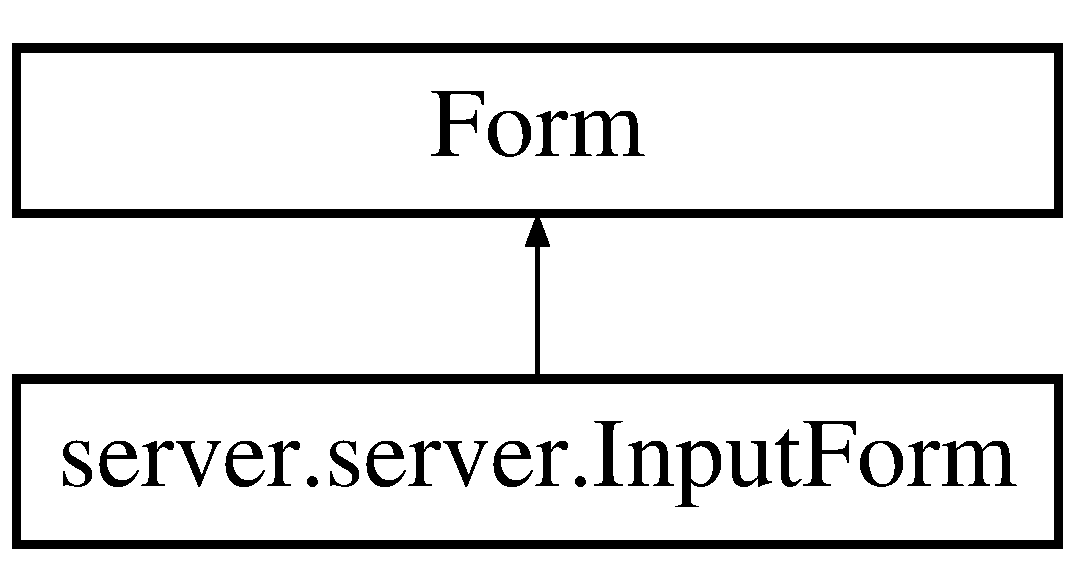
\includegraphics[height=2.000000cm]{classserver_1_1server_1_1_input_form}
\end{center}
\end{figure}
\subsection*{Static Public Attributes}
\begin{DoxyCompactItemize}
\item 
\mbox{\hyperlink{classserver_1_1server_1_1_input_form_ab4f0118c5e7a7ecc3ca50d7f781f2de2}{search\+\_\+query}} = String\+Field(u\textquotesingle{}Enter Your Search\+:\textquotesingle{}, render\+\_\+kw=\{\char`\"{}placeholder\char`\"{}\+: \char`\"{}Please Enter Queries as a Comma-\/Seperated list.\char`\"{}\}, validators = \mbox{[}validators.\+input\+\_\+required()\mbox{]})
\item 
\mbox{\hyperlink{classserver_1_1server_1_1_input_form_ad899681ccf68ae96f24ae575e3142635}{search\+\_\+state}} = Select\+Field(u\textquotesingle{}State\+:\textquotesingle{}, choices=\mbox{[}(\textquotesingle{}AL\textquotesingle{},\textquotesingle{}Alabama\textquotesingle{}), (\textquotesingle{}AK\textquotesingle{}, \textquotesingle{}Alaska\textquotesingle{}), (\textquotesingle{}AZ\textquotesingle{}, \textquotesingle{}Arizona\textquotesingle{}), (\textquotesingle{}AR\textquotesingle{}, \textquotesingle{}Arkansas\textquotesingle{}),(\textquotesingle{}CA\textquotesingle{}, \textquotesingle{}California\textquotesingle{}), (\textquotesingle{}CO\textquotesingle{}, \textquotesingle{}Colorado\textquotesingle{}), (\textquotesingle{}CT\textquotesingle{}, \textquotesingle{}Connecticut\textquotesingle{}), (\textquotesingle{}DE\textquotesingle{}, \textquotesingle{}Delaware\textquotesingle{}),(\textquotesingle{}FL\textquotesingle{}, \textquotesingle{}Florida\textquotesingle{}), (\textquotesingle{}GA\textquotesingle{}, \textquotesingle{}Georgia\textquotesingle{}), (\textquotesingle{}HI\textquotesingle{}, \textquotesingle{}Hawaii\textquotesingle{}), (\textquotesingle{}ID\textquotesingle{}, \textquotesingle{}Idaho\textquotesingle{}), (\textquotesingle{}IL\textquotesingle{}, \textquotesingle{}Illinois\textquotesingle{}), (\textquotesingle{}IN\textquotesingle{}, \textquotesingle{}Indiana\textquotesingle{}), (\textquotesingle{}IA\textquotesingle{}, \textquotesingle{}Iowa\textquotesingle{}), (\textquotesingle{}KS\textquotesingle{}, \textquotesingle{}Kansas\textquotesingle{}), (\textquotesingle{}KY\textquotesingle{}, \textquotesingle{}Kentucky\textquotesingle{}), (\textquotesingle{}LA\textquotesingle{}, \textquotesingle{}Louisiana\textquotesingle{}), (\textquotesingle{}ME\textquotesingle{}, \textquotesingle{}Maine\textquotesingle{}), (\textquotesingle{}MD\textquotesingle{}, \textquotesingle{}Maryland\textquotesingle{}), (\textquotesingle{}MA\textquotesingle{}, \textquotesingle{}Massachusetts\textquotesingle{}), (\textquotesingle{}MI\textquotesingle{}, \textquotesingle{}Michigan\textquotesingle{}), (\textquotesingle{}MN\textquotesingle{}, \textquotesingle{}Minnesota\textquotesingle{}), (\textquotesingle{}MS\textquotesingle{}, \textquotesingle{}Mississippi\textquotesingle{}), (\textquotesingle{}MO\textquotesingle{}, \textquotesingle{}Missouri\textquotesingle{}), (\textquotesingle{}MT\textquotesingle{}, \textquotesingle{}Montana\textquotesingle{}), (\textquotesingle{}NE\textquotesingle{}, \textquotesingle{}Nebraska\textquotesingle{}), (\textquotesingle{}NV\textquotesingle{}, \textquotesingle{}Nevada\textquotesingle{}), (\textquotesingle{}NH\textquotesingle{}, \textquotesingle{}New Hampshire\textquotesingle{}), (\textquotesingle{}NJ\textquotesingle{}, \textquotesingle{}New Jersey\textquotesingle{}), (\textquotesingle{}NM\textquotesingle{}, \textquotesingle{}New Mexico\textquotesingle{}), (\textquotesingle{}NY\textquotesingle{}, \textquotesingle{}New York\textquotesingle{}), (\textquotesingle{}NC\textquotesingle{}, \textquotesingle{}North Carolina\textquotesingle{}), (\textquotesingle{}ND\textquotesingle{}, \textquotesingle{}North Dakota\textquotesingle{}), (\textquotesingle{}OH\textquotesingle{}, \textquotesingle{}Ohio\textquotesingle{}), (\textquotesingle{}OK\textquotesingle{}, \textquotesingle{}Oklahoma\textquotesingle{}), (\textquotesingle{}OR\textquotesingle{}, \textquotesingle{}Oregon\textquotesingle{}), (\textquotesingle{}PA\textquotesingle{}, \textquotesingle{}Pennsylvania\textquotesingle{}), (\textquotesingle{}RI\textquotesingle{}, \textquotesingle{}Rhode Island\textquotesingle{}), (\textquotesingle{}SC\textquotesingle{}, \textquotesingle{}South Carolina\textquotesingle{}), (\textquotesingle{}SD\textquotesingle{}, \textquotesingle{}South Dakota\textquotesingle{}), (\textquotesingle{}TN\textquotesingle{}, \textquotesingle{}Tennessee\textquotesingle{}), (\textquotesingle{}TX\textquotesingle{}, \textquotesingle{}Texas\textquotesingle{}), (\textquotesingle{}UT\textquotesingle{}, \textquotesingle{}Utah\textquotesingle{}), (\textquotesingle{}VT\textquotesingle{}, \textquotesingle{}Vermont\textquotesingle{}), (\textquotesingle{}VA\textquotesingle{}, \textquotesingle{}Virginia\textquotesingle{}), (\textquotesingle{}WA\textquotesingle{}, \textquotesingle{}Washington\textquotesingle{}), (\textquotesingle{}WV\textquotesingle{}, \textquotesingle{}West Virginia\textquotesingle{}), (\textquotesingle{}WI\textquotesingle{}, \textquotesingle{}Wisconsin\textquotesingle{}), (\textquotesingle{}WY\textquotesingle{}, \textquotesingle{}Wyoming\textquotesingle{})\mbox{]}, default=\textquotesingle{}KS\textquotesingle{})
\item 
\mbox{\hyperlink{classserver_1_1server_1_1_input_form_a219d510984378b86ca3c87003cba3ab2}{search\+\_\+city}} = String\+Field(u\textquotesingle{}City\+:\textquotesingle{}, validators = \mbox{[}validators.\+input\+\_\+required()\mbox{]}, default=\char`\"{}Lawrence\char`\"{})
\end{DoxyCompactItemize}


\subsection{Detailed Description}
C\+L\+A\+S\+S\+ES. 

\mbox{\hyperlink{classserver_1_1server_1_1_input_form}{Input\+Form}}

Form that Takes the String(s) Given as Input and passes them into the dictionary See W\+T\+Forms Documentation for more information regarding declaration of form classes and their params 

\subsection{Member Data Documentation}
\mbox{\Hypertarget{classserver_1_1server_1_1_input_form_a219d510984378b86ca3c87003cba3ab2}\label{classserver_1_1server_1_1_input_form_a219d510984378b86ca3c87003cba3ab2}} 
\index{server\+::server\+::\+Input\+Form@{server\+::server\+::\+Input\+Form}!search\+\_\+city@{search\+\_\+city}}
\index{search\+\_\+city@{search\+\_\+city}!server\+::server\+::\+Input\+Form@{server\+::server\+::\+Input\+Form}}
\subsubsection{\texorpdfstring{search\+\_\+city}{search\_city}}
{\footnotesize\ttfamily server.\+server.\+Input\+Form.\+search\+\_\+city = String\+Field(u\textquotesingle{}City\+:\textquotesingle{}, validators = \mbox{[}validators.\+input\+\_\+required()\mbox{]}, default=\char`\"{}Lawrence\char`\"{})\hspace{0.3cm}{\ttfamily [static]}}

\mbox{\Hypertarget{classserver_1_1server_1_1_input_form_ab4f0118c5e7a7ecc3ca50d7f781f2de2}\label{classserver_1_1server_1_1_input_form_ab4f0118c5e7a7ecc3ca50d7f781f2de2}} 
\index{server\+::server\+::\+Input\+Form@{server\+::server\+::\+Input\+Form}!search\+\_\+query@{search\+\_\+query}}
\index{search\+\_\+query@{search\+\_\+query}!server\+::server\+::\+Input\+Form@{server\+::server\+::\+Input\+Form}}
\subsubsection{\texorpdfstring{search\+\_\+query}{search\_query}}
{\footnotesize\ttfamily server.\+server.\+Input\+Form.\+search\+\_\+query = String\+Field(u\textquotesingle{}Enter Your Search\+:\textquotesingle{}, render\+\_\+kw=\{\char`\"{}placeholder\char`\"{}\+: \char`\"{}Please Enter Queries as a Comma-\/Seperated list.\char`\"{}\}, validators = \mbox{[}validators.\+input\+\_\+required()\mbox{]})\hspace{0.3cm}{\ttfamily [static]}}

\mbox{\Hypertarget{classserver_1_1server_1_1_input_form_ad899681ccf68ae96f24ae575e3142635}\label{classserver_1_1server_1_1_input_form_ad899681ccf68ae96f24ae575e3142635}} 
\index{server\+::server\+::\+Input\+Form@{server\+::server\+::\+Input\+Form}!search\+\_\+state@{search\+\_\+state}}
\index{search\+\_\+state@{search\+\_\+state}!server\+::server\+::\+Input\+Form@{server\+::server\+::\+Input\+Form}}
\subsubsection{\texorpdfstring{search\+\_\+state}{search\_state}}
{\footnotesize\ttfamily server.\+server.\+Input\+Form.\+search\+\_\+state = Select\+Field(u\textquotesingle{}State\+:\textquotesingle{}, choices=\mbox{[}(\textquotesingle{}AL\textquotesingle{},\textquotesingle{}Alabama\textquotesingle{}), (\textquotesingle{}AK\textquotesingle{}, \textquotesingle{}Alaska\textquotesingle{}), (\textquotesingle{}AZ\textquotesingle{}, \textquotesingle{}Arizona\textquotesingle{}), (\textquotesingle{}AR\textquotesingle{}, \textquotesingle{}Arkansas\textquotesingle{}),(\textquotesingle{}CA\textquotesingle{}, \textquotesingle{}California\textquotesingle{}), (\textquotesingle{}CO\textquotesingle{}, \textquotesingle{}Colorado\textquotesingle{}), (\textquotesingle{}CT\textquotesingle{}, \textquotesingle{}Connecticut\textquotesingle{}), (\textquotesingle{}DE\textquotesingle{}, \textquotesingle{}Delaware\textquotesingle{}),(\textquotesingle{}FL\textquotesingle{}, \textquotesingle{}Florida\textquotesingle{}), (\textquotesingle{}GA\textquotesingle{}, \textquotesingle{}Georgia\textquotesingle{}), (\textquotesingle{}HI\textquotesingle{}, \textquotesingle{}Hawaii\textquotesingle{}), (\textquotesingle{}ID\textquotesingle{}, \textquotesingle{}Idaho\textquotesingle{}), (\textquotesingle{}IL\textquotesingle{}, \textquotesingle{}Illinois\textquotesingle{}), (\textquotesingle{}IN\textquotesingle{}, \textquotesingle{}Indiana\textquotesingle{}), (\textquotesingle{}IA\textquotesingle{}, \textquotesingle{}Iowa\textquotesingle{}), (\textquotesingle{}KS\textquotesingle{}, \textquotesingle{}Kansas\textquotesingle{}), (\textquotesingle{}KY\textquotesingle{}, \textquotesingle{}Kentucky\textquotesingle{}), (\textquotesingle{}LA\textquotesingle{}, \textquotesingle{}Louisiana\textquotesingle{}), (\textquotesingle{}ME\textquotesingle{}, \textquotesingle{}Maine\textquotesingle{}), (\textquotesingle{}MD\textquotesingle{}, \textquotesingle{}Maryland\textquotesingle{}), (\textquotesingle{}MA\textquotesingle{}, \textquotesingle{}Massachusetts\textquotesingle{}), (\textquotesingle{}MI\textquotesingle{}, \textquotesingle{}Michigan\textquotesingle{}), (\textquotesingle{}MN\textquotesingle{}, \textquotesingle{}Minnesota\textquotesingle{}), (\textquotesingle{}MS\textquotesingle{}, \textquotesingle{}Mississippi\textquotesingle{}), (\textquotesingle{}MO\textquotesingle{}, \textquotesingle{}Missouri\textquotesingle{}), (\textquotesingle{}MT\textquotesingle{}, \textquotesingle{}Montana\textquotesingle{}), (\textquotesingle{}NE\textquotesingle{}, \textquotesingle{}Nebraska\textquotesingle{}), (\textquotesingle{}NV\textquotesingle{}, \textquotesingle{}Nevada\textquotesingle{}), (\textquotesingle{}NH\textquotesingle{}, \textquotesingle{}New Hampshire\textquotesingle{}), (\textquotesingle{}NJ\textquotesingle{}, \textquotesingle{}New Jersey\textquotesingle{}), (\textquotesingle{}NM\textquotesingle{}, \textquotesingle{}New Mexico\textquotesingle{}), (\textquotesingle{}NY\textquotesingle{}, \textquotesingle{}New York\textquotesingle{}), (\textquotesingle{}NC\textquotesingle{}, \textquotesingle{}North Carolina\textquotesingle{}), (\textquotesingle{}ND\textquotesingle{}, \textquotesingle{}North Dakota\textquotesingle{}), (\textquotesingle{}OH\textquotesingle{}, \textquotesingle{}Ohio\textquotesingle{}), (\textquotesingle{}OK\textquotesingle{}, \textquotesingle{}Oklahoma\textquotesingle{}), (\textquotesingle{}OR\textquotesingle{}, \textquotesingle{}Oregon\textquotesingle{}), (\textquotesingle{}PA\textquotesingle{}, \textquotesingle{}Pennsylvania\textquotesingle{}), (\textquotesingle{}RI\textquotesingle{}, \textquotesingle{}Rhode Island\textquotesingle{}), (\textquotesingle{}SC\textquotesingle{}, \textquotesingle{}South Carolina\textquotesingle{}), (\textquotesingle{}SD\textquotesingle{}, \textquotesingle{}South Dakota\textquotesingle{}), (\textquotesingle{}TN\textquotesingle{}, \textquotesingle{}Tennessee\textquotesingle{}), (\textquotesingle{}TX\textquotesingle{}, \textquotesingle{}Texas\textquotesingle{}), (\textquotesingle{}UT\textquotesingle{}, \textquotesingle{}Utah\textquotesingle{}), (\textquotesingle{}VT\textquotesingle{}, \textquotesingle{}Vermont\textquotesingle{}), (\textquotesingle{}VA\textquotesingle{}, \textquotesingle{}Virginia\textquotesingle{}), (\textquotesingle{}WA\textquotesingle{}, \textquotesingle{}Washington\textquotesingle{}), (\textquotesingle{}WV\textquotesingle{}, \textquotesingle{}West Virginia\textquotesingle{}), (\textquotesingle{}WI\textquotesingle{}, \textquotesingle{}Wisconsin\textquotesingle{}), (\textquotesingle{}WY\textquotesingle{}, \textquotesingle{}Wyoming\textquotesingle{})\mbox{]}, default=\textquotesingle{}KS\textquotesingle{})\hspace{0.3cm}{\ttfamily [static]}}



The documentation for this class was generated from the following file\+:\begin{DoxyCompactItemize}
\item 
\mbox{\hyperlink{server_8py}{server.\+py}}\end{DoxyCompactItemize}

\chapter{File Documentation}
\hypertarget{____init_____8py}{}\section{\+\_\+\+\_\+init\+\_\+\+\_\+.\+py File Reference}
\label{____init_____8py}\index{\+\_\+\+\_\+init\+\_\+\+\_\+.\+py@{\+\_\+\+\_\+init\+\_\+\+\_\+.\+py}}
\subsection*{Namespaces}
\begin{DoxyCompactItemize}
\item 
 \mbox{\hyperlink{namespaceserver_1_1_scraper}{server.\+Scraper}}
\end{DoxyCompactItemize}

\hypertarget{server_8py}{}\section{server.\+py File Reference}
\label{server_8py}\index{server.\+py@{server.\+py}}


Server run File that provides the main interface between our app and th Server Includes routing Information and Rendering of H\+T\+ML.  


\subsection*{Classes}
\begin{DoxyCompactItemize}
\item 
class \mbox{\hyperlink{classserver_1_1server_1_1_input_form}{server.\+server.\+Input\+Form}}
\begin{DoxyCompactList}\small\item\em C\+L\+A\+S\+S\+ES. \end{DoxyCompactList}\end{DoxyCompactItemize}
\subsection*{Namespaces}
\begin{DoxyCompactItemize}
\item 
 \mbox{\hyperlink{namespaceserver_1_1server}{server.\+server}}
\item 
 \mbox{\hyperlink{namespace_flask}{Flask}}
\begin{DoxyCompactList}\small\item\em Documentation for the Server \mbox{\hyperlink{namespace_flask}{Flask}} is a Microframework for Web Development thtat Utilizes Python. \end{DoxyCompactList}\end{DoxyCompactItemize}
\subsection*{Functions}
\begin{DoxyCompactItemize}
\item 
def \mbox{\hyperlink{namespaceserver_1_1server_a59e9bd350bd3f6864626e826a5d07e61}{server.\+server.\+Handle\+Data}} (data)
\begin{DoxyCompactList}\small\item\em Handle \end{DoxyCompactList}\item 
def \mbox{\hyperlink{namespaceserver_1_1server_a06b6b48a36458a5e63d37667433c2080}{server.\+server.\+Create\+Dict}} (name)
\begin{DoxyCompactList}\small\item\em Function. \end{DoxyCompactList}\item 
def \mbox{\hyperlink{namespaceserver_1_1server_ab3d96b92729f42de2866e0cb876a0a71}{server.\+server.\+index}} ()
\begin{DoxyCompactList}\small\item\em R\+O\+U\+T\+ES. \end{DoxyCompactList}\item 
def \mbox{\hyperlink{namespaceserver_1_1server_ae5d697d5408aeb2f94e2aa610a4706aa}{server.\+server.\+search}} ()
\item 
def \mbox{\hyperlink{namespaceserver_1_1server_a7bdc96668852473d18262dd1185ac3d9}{server.\+server.\+about}} ()
\begin{DoxyCompactList}\small\item\em Function \char`\"{}/about\char`\"{}. \end{DoxyCompactList}\item 
def \mbox{\hyperlink{namespaceserver_1_1server_a83a8086e94730016efda959e40b9cfaf}{server.\+server.\+results}} ()
\end{DoxyCompactItemize}
\subsection*{Variables}
\begin{DoxyCompactItemize}
\item 
\mbox{\hyperlink{namespaceserver_1_1server_abe540ab6e7c9bffd61dda91273e699e2}{server.\+server.\+app}} = Flask(\+\_\+\+\_\+name\+\_\+\+\_\+, static\+\_\+folder=\char`\"{}../static/dist\char`\"{}, template\+\_\+folder=\char`\"{}../static\char`\"{})
\item 
\mbox{\hyperlink{namespaceserver_1_1server_addf5a8b97b626d4622f3fb2b2f8065ab}{server.\+server.\+debug}}
\item 
\mbox{\hyperlink{namespaceserver_1_1server_a1e0984522028dec04483b66d00e8b6b6}{server.\+server.\+methods}}
\begin{DoxyCompactList}\small\item\em Class \char`\"{}/search\char`\"{}. \end{DoxyCompactList}\item 
\mbox{\hyperlink{namespaceserver_1_1server_a70d8440bb9056abff06b917ecacce061}{server.\+server.\+secret\+\_\+key}}
\begin{DoxyCompactList}\small\item\em Runs the Server. \end{DoxyCompactList}\end{DoxyCompactItemize}


\subsection{Detailed Description}
Server run File that provides the main interface between our app and th Server Includes routing Information and Rendering of H\+T\+ML. 

Runs the Landscrape Main Server.
%--- End generated contents ---

% Index
\backmatter
\newpage
\phantomsection
\clearemptydoublepage
\addcontentsline{toc}{chapter}{Index}
\printindex

\end{document}
